\chapter{Literature Review}

This chapter reviews the currently available implementations of various
components in the processing pipeline. The first two sections enumerate
the two relevant pipelines --- Section~\ref{sec:lr:trans} describes
transcription, and Section~\ref{sec:lr:cap} describes captioning.
Finally, Section 2.3~\ref{sec:lr:summ} summarises the various implementations.

Most of the implementations chosen are free, open-source and cross-platform.

\section{Transcription}\label{sec:lr:trans}

Figure~\ref{trans} provided the transcription pipeline of three components
--- a resampler, a diarizer and a transcription engine. We would go into
each component in detail.

Furthermore, to enable transcription of multi-channel recording, the concept
of voice-activity detection (VAD) would also be discussed.

\subsection{Resampling}\label{resampling}

In the context of this project, resampling is concerned with converting an
audio stream from different specifications to a standard one, before passing to
other processing steps. Table~\ref{audio} describes some common attributes
of an audio stream.

\begin{longtabu}{X[1.5,l]X[4,l]X[2.5,l]}
    \textbf{Attribute} & \textbf{Description} & \textbf{Examples} \\
    \midrule
    \endhead{}
    Sample rate &
    (defined for PCM audio)\newline Number of audio samples per
    second~\cite{weik1995communications} &
    CD audio: 44100 Hz~\cite{cd} \\
    Bit depth &
    (defined for PCM audio)\newline Number of bits to represent
    a sample~\cite{thompson2005understanding} &
    CD audio: 16 bits~\cite{cd} \\
    Number of channels &
    Number of independent audio channels (to create a
    perception of depth) &
    Mono (1-channel)/\newline
    Stereo (2-channel)~\cite{mono-stereo} \\
    Audio coding format &
    The specific encoder/ decoder used to create the audio stream;
    usually associated with a certain file extension &
    MPEG-2 Audio Layer III (\texttt{.mp3})~\cite{mp3}\newline
    WAVE (\texttt{.wav})~\cite{wav} \\
    \caption{Common audio stream attributes}\label{audio}
\end{longtabu}

Respectively, in order to resample audio streams, the following tasks
are performed on the original audio stream\footnote{The canonical
definition of resampling is only concerned with the first task
(sample rate conversion).}:

\begin{itemize}
    \item Sample rate conversion --- changing the sample rate of the audio
    (for instance, from 44100Hz to 16000Hz)
    \item Sample format conversion --- changing the type of the sample
    (for instance, from 16-bit to 8-bit samples)
    \item Channel rematrixing --- changing the number of channels
    (for instance, from stereo to mono audio)
    \item Transcoding --- changing the audio coding format (for instance,
    from WAVE to MPEG Layer-III)
\end{itemize}

There are two software packages to perform all the above tasks:

\subsubsection{Sound eXchange --- SoX (\texttt{sox})}

SoX is a cross-platform command-line utility that supports conversion
between a wide range of audio formats. Additionally, the utility could
apply effects, and play and record audio files~\cite{sox-docs}.
SoX is written in C\@; the associated library is \texttt{libsox}. Its
resampling library is released separately as
\texttt{libsoxr}~\cite{sox}.

Figure~\ref{sox} shows an example run of SoX.

\begin{figure}[ht]
\begin{center}
    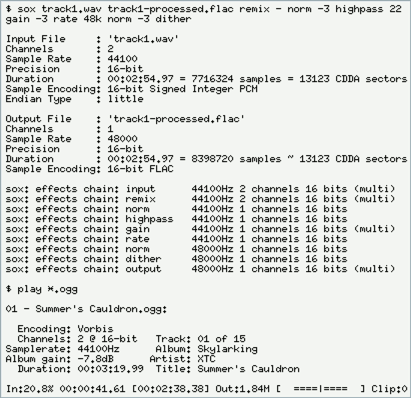
\includegraphics[width=0.6\textwidth]{sox}
    \caption{An example SoX session~\cite{sox}}\label{sox}
\end{center}
\end{figure}

The latest version of SoX, 14.4.2 was released in February 2015. The
current status of development work is uncertain; many issues and pull
requests are outstanding~\cite{sox-cl}.

\subsubsection{FFmpeg (\texttt{ffmpeg})}

FFmpeg is another C cross-platform utility to record, convert and stream
audio and video~\cite{ffmpeg}. FFmpeg provides a resampler which can
perform audio resampling, audio channel layout rematrixing, and convert
audio format and packing layout; it interfaces with its own resampling
library (\texttt{libswresample}) as well as SoX's resampling
library~\cite{ffmpeg-res,ffmpeg-libres}.

The library is actively developed; its latest stable version is 3.4
and it was released in October 2017~\cite{ffmpeg-dl}.

\subsubsection{Evaluation}

The two packages offer very similar functionalities; they are also
highly performant. However, FFmpeg has two clear advantages: it is
actively maintained and updated, and it operates on both audio and
video files (compare to audio only for SoX). FFmpeg also supports
more audio formats out-of-the-box.

Overall, FFmpeg would be a more suitable package for the project.

\subsection{Diarization}

With respect to an audio stream of multiple speakers, diarization is
the process of determining which speaker is speaking at when~\cite{diar}. 
Diarization is a combination of two tasks --- speaker segmentation,
which is the process of finding speaker change points in an audio stream,
to split the stream into smaller segments; and speaker clustering,
which is the process of grouping said segments based on speaker
characteristics, ideally resulting in one cluster per actual
speaker~\cite{diar-cls}.

Implementations of speaker diarization usually follow one of these
two approaches~\cite{diar}:

\begin{itemize}
    \item Bottom-up --- initialize a large number of segments (more than
    the optimal), then iteratively merge segments until optimal
    \item Top-down --- initialize a single model of one segment (the whole
    audio stream), then iteratively add new models corresponding to new
    segments, until optimal
\end{itemize}

Both are characterised by the use of Hidden Markov Models (HMMs) and 
Gaussian Mixture Models (GMMs), a statiscal and probabilistic approach
to clustering.

One of the most frequently cited diarization toolkit is LIUM Speaker
Diarization.

\subsubsection{LIUM Speaker Diarization}

LIUM Speaker Diarization is an open-source diarization toolkit developed
at Laboratoire d'Informatique de l'Université du Maine~\cite{lium}.

\begin{figure}[h]
\begin{center}
    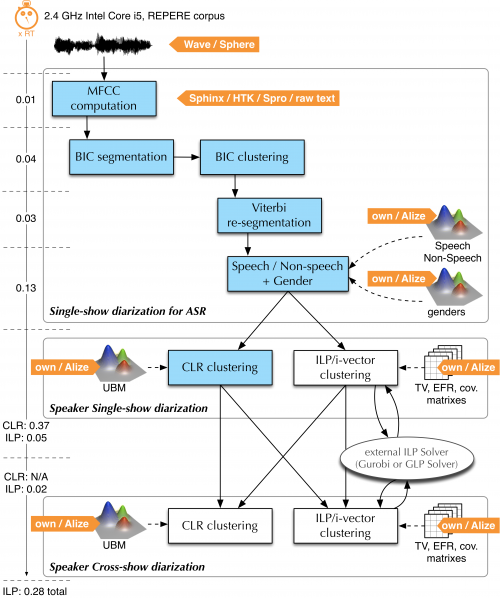
\includegraphics[width=0.6\textwidth]{diarization}
    \caption{The LIUM processing pipeline~\cite{lium-ovr}}\label{lium}
\end{center}
\end{figure}

Figure~\ref{lium} outlines the steps in LIUM's processing pipeline.
LIUM follows the bottom-up approach; it utilises agglomerative hierarchical
clustering, using Bayesian Information Criterion as the stopping/ clustering
criteria. LIUM produces a segmentation file (\texttt{.seg}) which details
the start time, length and \texttt{speaker\_id} of all identified
segments. An example segmentation is shown in Figure~\ref{seg}\footnote{The
segmentation output has 8 fields, in this particular
order: \texttt{show\_id}, \texttt{channel\_id}, start time, length, gender
type of band, type of environment and \texttt{speaker\_id}.}~\cite{lium-seg}.

\begin{figure}[h]
\begin{lstlisting}
20071218_1900_1920_inter 1 0    322   M S U S0
20071218_1900_1920_inter 1 322  680   F S U S1
20071218_1900_1920_inter 1 1148 371   M S U S143
20071218_1900_1920_inter 1 1772 310   F S U S3
20071218_1900_1920_inter 1 2082 318   F S U S28
20071218_1900_1920_inter 1 2495 1570  M S U S12
\end{lstlisting}
\caption{Sample segmentation output}\label{seg}
\end{figure}

LIUM is written in Java; however there is a convenient CLI~\cite{lium}
utilising its \texttt{.jar} package.
Its latest version is 8.4.1, released in September 2013~\cite{lium-dl}.

\subsubsection{Evaluation}

LIUM is considered one of the state-of-the-art toolkits in speaker
diarization; it came out on top in a series of evaluations~\cite{lium-ester,
lium-revere}. It is also very performant, as evidence in Figure~\ref{lium}:
using relatively recent hardware, it takes less than half-real-time
to diarize an audio stream. It also does a good job of preparing the
audio stream for ASR\@: resulting segments are short and single-speaker.

However, the out-of-the-box configuration is tuned towards broadcast
news diarization; for other audio domains the results might vary
and specific tuning might be required. The toolkit is also fairly outdated.

Nonetheless, LIUM is a great starting point for building the diarization
component for the transcription processing pipeline. 

\subsection{Transcription Engine}

The main purpose of the transcription engine is to transcribe speech
segments to text (in other words, to perform ASR). 

Figure~\ref{asr} outlines the typical architecture of an ASR
system. The ASR system takes in an audio stream and extract
its features --- the most common being mel-frequency cepstral
coeffcients (MFCCs) --- then pass the features to an acoustic model.
Combined with a language model, the ASR system comes up with probable
results and selects the best one based on its criteria~\cite{asr}.

\begin{figure}[h]
\begin{center}
    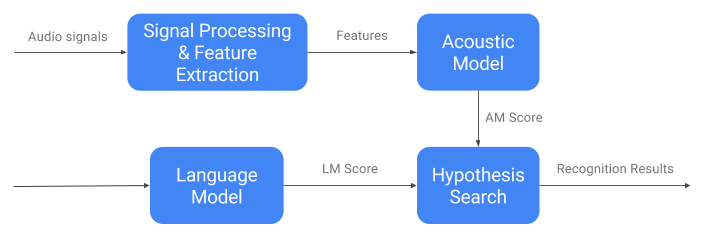
\includegraphics[width=0.9\textwidth]{pipeline_asr}
    \caption{Structure of an ASR system}\label{asr}
\end{center}
\end{figure}

The current state-of-the-art in ASR are among these two methodologies:

\begin{itemize}
    \item Statiscal/ probabilistic methods, utilising a combination of
    HMMs and GMMs
    \item Deep neural network (DNN)-based methods
\end{itemize}

With the advent of high-performance computing, DNN-based methods are
quickly gaining traction. We review two DNN-based transcription engines.

\subsubsection{Google Cloud Speech API}

Cloud Speech API is developed by Google, providing the same speech
recognition capabilities powering Google's native applications (such as
Google Voice Search and Google Assistant) to developers. Cloud Speech API
has support for 110 languages, including multiple variances of popular
languages such as English~\cite{gcs}.

The implementation details of Cloud Speech API are hidden to the developer;
various API libraries\footnote{Most of the libraries are experimental and
continuously updated.} for common programming languages are
provided~\cite{gcs-libs}. In a normal workflow, speech segments are sent to
Google's servers through the client libraries in one of three configurations:
synchronous, asynchronous and streaming recognition; the servers return
recognition results in JSON\@. A sample is given in Figure~\ref{gcs}.

\begin{figure}[ht]
\begin{lstlisting}
    {
        "results": [
            {
                "alternatives": [
                    {
                        "transcript": "how old is the Brooklyn Bridge",
                        "confidence": 0.98267895
                    }
                ]
            }
        ]
    }      
\end{lstlisting}
\caption{Sample Google Cloud Speech API recognition result}\label{gcs}
\end{figure}

To perform speech recognition, one needs to provide
a Google API service account key~\cite{gcs-api-key} and this key is used
for usage tracking; the free tier only allows \$300 of credits to be used
in 12 months~\cite{gcs-free}\footnote{Usage is charged in terms of 15-second
blocks; each block is \$0.0025.}.

\subsubsection{Kaldi}

Kaldi is an open-source toolkit for speech recognition, developed with a
goal of being modern and flexible, to allow for easy extension and
modification.

Figure~\ref{kaldi} outlines the structure of Kaldi. It is a collection of
command-line tools written in C++ that rely on standard numerical
algebra (BLAS/LAPACK) and finite state transducer (OpenFST) libraries,
and shell scripts to pipe the tools together to build a complete ASR
system. Recipes and data are provided for a large number of ASR and DNN
tasks~\cite{kaldi}.

\begin{figure}[h]
\begin{center}
    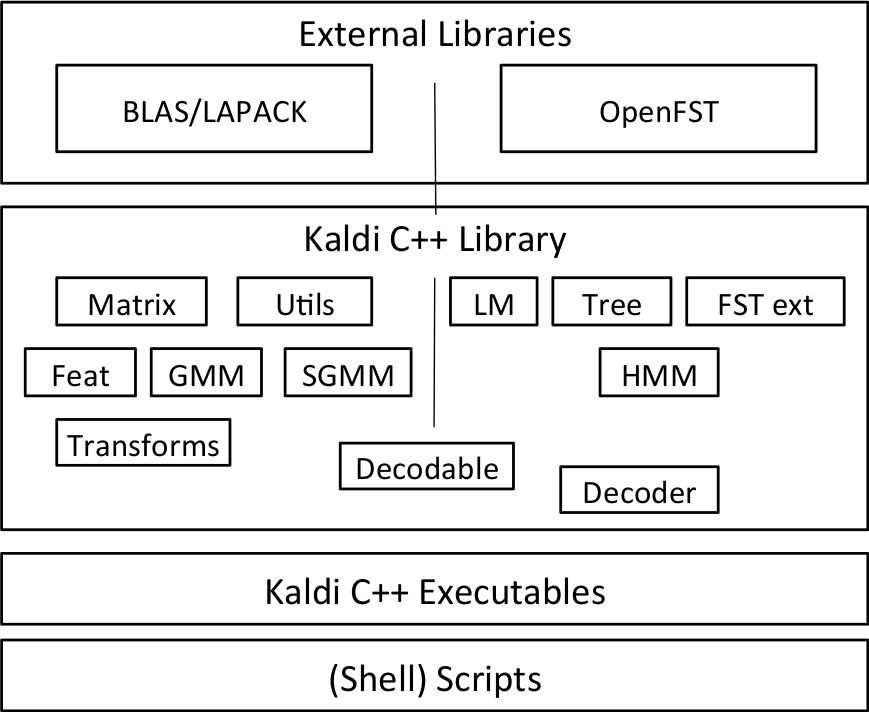
\includegraphics[width=0.6\textwidth]{kaldi-lib}
    \caption{Structure of Kaldi}\label{kaldi}
\end{center}
\end{figure}

Kaldi is actively developed; the developers encourage Kaldi users to
check out the latest version of Kaldi available~\cite{kaldi-ver}.

\subsubsection{Evaluation}

Both Google Cloud Speech API and Kaldi are DNN-based ASR systems considered
state-of-the-art in commercial~\cite{gcs-comp} and open-source~\cite{kaldi-comp}
communities respectively. Both systems are continuously updated and improved;
however as a commercial solution, Google Cloud Speech API's underlying model
improvements are invisible to developers, and the system is technically not
free. Kaldi makes it easier to tweak and design an ASR system on the ground up.

There is an interest to compare both systems' performance on a real-world
scenario; the project would attempt to run both Google Cloud Speech API
and Kaldi.

\subsection{Voice-activity Detection (VAD)}

VAD is defined as the process to distinguish speech from non-speech segments.
It is fundamental for a speech processing system to perform VAD well, otherwise
time and computational power would be wasted on processing non-speech
segments~\cite{vad}.

A reference structure to perform VAD is describe in Figure~\ref{vad}~\cite{vad}.
Features are extracted from the raw signals; the features should differentiate
speech and non-speech well. Different features already explored in literature
include power and signal-to-noise, pitch and harmonicity, stationarity and
modulation~\cite{vad-feats}. Features are then passed to a decision module to
produce an initial VAD decision, which is then smoothed to a final decision.

\begin{figure}[h]
\begin{center}
    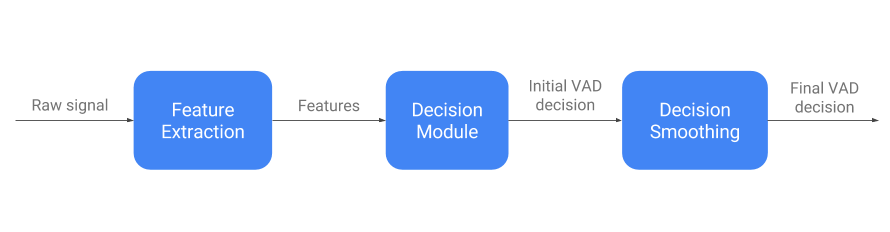
\includegraphics[width=0.9\textwidth]{pipeline_vad}
    \caption{Structure of a VAD system}\label{vad}
\end{center}
\end{figure}

We are interested in the scenario of a multi-channel recording. In such a
scenario, multiple speakers might be speaking concurrently to individual
close-talk microphones\footnote{A close-talk microphone is one designed to pick
up voices from a very close distance (10cm or less).}. Despite the use of such
microphones, the problem of crosstalk persists; in a particular speaker's
close-talk recording, speech segments from other speakers still exist, and
their presence would interfere with attempts to do ASR on the
recording~\cite{vad-mc}. Multi-channel VAD attempts
to remove the crosstalk before passing the (clean) speech to an ASR system.

\section{Captioning}\label{sec:lr:cap}

Figure~\ref{cap} provided the image captioning pipeline of two components ---
a converter and a caption generator. We would go into each component in detail.

\subsection{Video conversion}

Similar to the process of resampling described in Section~\ref{resampling},
conversion is concerned with changing a video file from different specifications
to a standard one before passing to other processing steps. A video file
is a container, containing a video stream as well as one or more audio
streams, and usually associated with an extension~\cite{vid}.

Some of the most common container formats include:

\begin{itemize}
    \item Audio-Video Interleave (\texttt{.avi}), developed by
    Microsoft~\cite{avi} and is the default format playable in Windows
    \item Flash Video (\texttt{.flv}), developed by Adobe~\cite{flv} and is
    the most common streaming format up until recent years
    \item MPEG-4 Part 14 (\texttt{.mp4}), developed as a standard by the
    Moving Pictures Experts Group~\cite{mp4}, considered the current
    \textit{de facto} video format.
\end{itemize}

Depending on the container format, the video and audio streams could be permitted
to follow different specific video/audio formats. Given a source and a target
container format, the conversion process could proceed as per Figure~\ref{convert}.
The source container would be unpacked to its individual audio/ video streams.
The streams would be resampled/ re-encoded depending on the target container, then
packed together in the target container format.

\begin{figure}[ht]
\begin{center}
    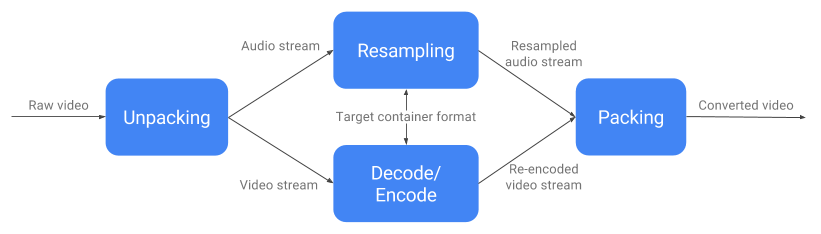
\includegraphics[width=0.9\textwidth]{pipeline_convert}
    \caption{Video conversion pipeline}\label{convert}
\end{center}
\end{figure}

Similar to Section~\ref{resampling}, the open-source toolkit of choice to handle
video conversion is FFmpeg. It provides two libraries, \texttt{libavcodec} and
\texttt{libavformat}, generic frameworks for encoding/ decoding streams, and
multiplexing/ demultiplexing container formats~\cite{ffmpeg-libav, ffmpeg-libfmt}.

\subsection{Caption generation}

Generating human-like description of images is an important and difficult task
in artificial intelligence, that merges computer vision and NLP --- a caption
generator must be able to recognize, separate and describe objects in an image,
and it must be able to string the individual descriptions together in a natural
way to achieve human-like performance~\cite{google-img,nrtalk}.

Recently, the state-of-the-art approaches to caption generation are DNN-based;
they combine a DNN approach to computer vision with another DNN approach in
natural language processing. The recent availability of large, annotated
image datasets such as ImageNet, Flickr8K, Flickr30K and MSCOCO~\cite{imagenet,
flickr8k,flickr30k,mscoco} also aids the rapid advancements in this field.

We briefly review two DNN-based approaches. Their overall structure is similar
to the one described in Figure~\ref{dnn-cap}; in the training phase, the training
dataset with images and human captions would go through DNNs to learn objects
and their relations, and produce a model which would be applied on a test set
of unseen images. The generated caption would be compared with the ``gold truth''
and scored using a number of metrics.

\begin{figure}[ht]
\begin{center}
    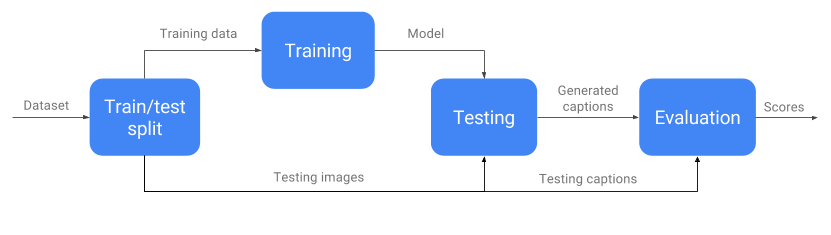
\includegraphics[width=0.9\textwidth]{pipeline_caption}
    \caption{DNN-based caption generation pipeline}\label{dnn-cap}
\end{center}
\end{figure}

The two approaches only differ in their choice of DNN architecture.

\subsubsection{NeuralTalk}

NeuralTalk~\cite{nrtalk} is an image captioning system developed by researchers
at Stanford University. The system is a combination of convolutional neural
networks (CNNs)\footnote{CNN is a DNN architecture utilising a number of
convolution and pooling layers to reduce the dimensions of high-dimensional
features such as images. It is considered the state-of-the-art for image-related
tasks.} on image regions, recurrent neural networks (RNNs)\footnote{RNN is a DNN
architecture where the input to the next layer is the output of previous layers
(hence the name ``recurrent''). It is considered the state-of-the-art in
sequential data processing, such as in NLP tasks.} on the captions, and a
multimodal embedding to align the two DNN structures.

The original implementation is open-source and available online; an updated
version, NeuralTalk2, is also available~\cite{gh-nrtalk,gh-nrtalk2}.

\subsubsection{Google Neural Image Captioning}

Neural Image Captioning~\cite{google-img} is developed by researchers at Google.
The system combines CNNs for encoding image features and long short-term memory
(LSTM)\footnote{LSTM is a special type of RNN that could``remember'' values over
arbitrary intervals, unlike normal RNNs where values change over time due to
training by gradient-descent. The special structure leads to higher performance
in the same tasks that RNNs excel in, i.e.\ NLP tasks.} networks for processing
captions.

The original implementation is also open-source and available
online~\cite{gh-google-img}.

\subsubsection{Evaluation}

Both systems are state-of-the-art and performs very well in standardised
image captioning challenges\cite{nrtalk,google-img}. However, such results do
not necessarily translate to real-world applications; it is unclear how well
they would perform on new images that are not in any dataset. The training
process is also prohibitively long without the use of graphical processing
units (GPUs); even with GPUs training time is still very long, owing to the 
complexity of DNN calculations. A pretrained model would be useful to reduce
the time taken to build a solution based on these methods.

\section{Summary}\label{sec:lr:summ}

In this chapter, we have presented a brief review of current frameworks to
address individual components of the transcription and captioning pipelines:
resampling (FFmpeg, SoX), diarization (LIUM), transcription engines (Google
Cloud Speech API, Kaldi), multi-channel VAD, video conversion (FFmpeg) and
caption generation (NeuralTalk and Google Neural Image Captioning). We have
seen that realising individual components is a relatively easy task; there
are an abundance of tools available to address specific problems. The hard
question remains: how to connect the tools together to build a complete
system for the specified task.

The next two chapters would present the system developed to achieve the
goal.
